% !TeX root = ../memoria.tex
\chapter{Curvas de desviación de Allan de la IMU}
\label{anexo:allan}

En este anexo se recogen las curvas de desviación de Allan obtenidas para los tres ejes del
acelerómetro y los tres ejes del giróscopo. Estas curvas se emplearon para estimar los
parámetros de ruido blanco \(N\) y paseo aleatorio del sesgo \(K\) utilizados en la
configuración del estimador VIO.

\begin{figure}[p]
    \centering
    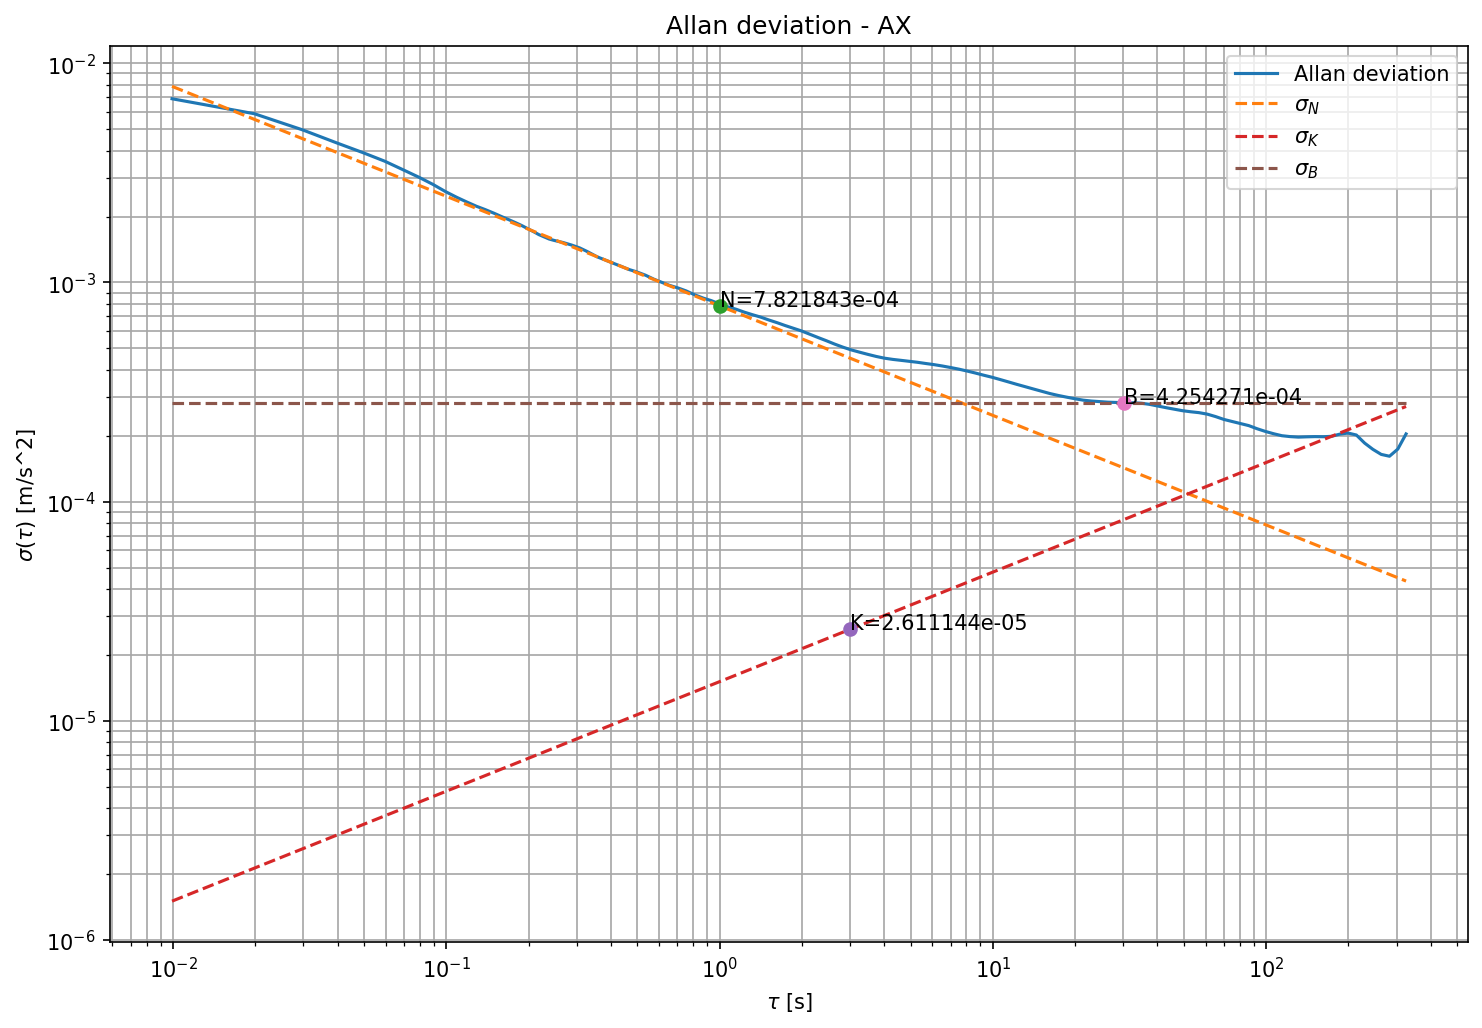
\includegraphics[width=0.88\textwidth]{images/ax_allan.png}
    \caption{Curva de desviación de Allan correspondiente al eje \(x\) del acelerómetro durante el ensayo estático de una hora.}
    \label{fig:allan_ax_anexo}
\end{figure}

\begin{figure}[p]
    \centering
    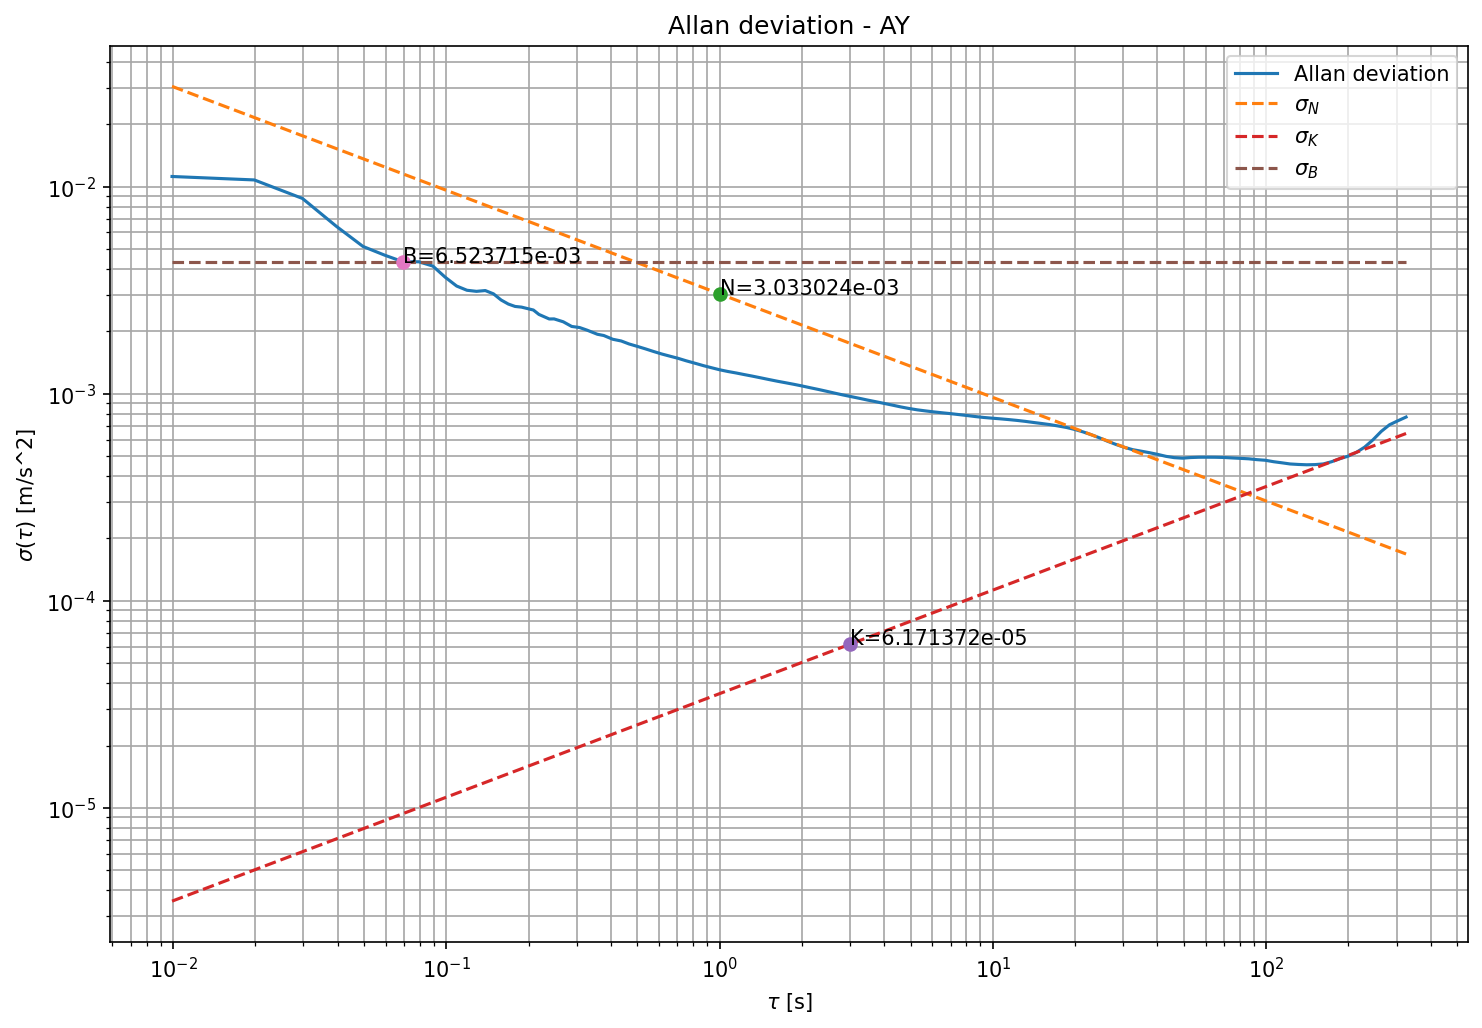
\includegraphics[width=0.88\textwidth]{images/ay_allan.png}
    \caption{Curva de desviación de Allan correspondiente al eje \(y\) del acelerómetro durante el ensayo estático de una hora.}
    \label{fig:allan_ay_anexo}
\end{figure}

\begin{figure}[p]
    \centering
    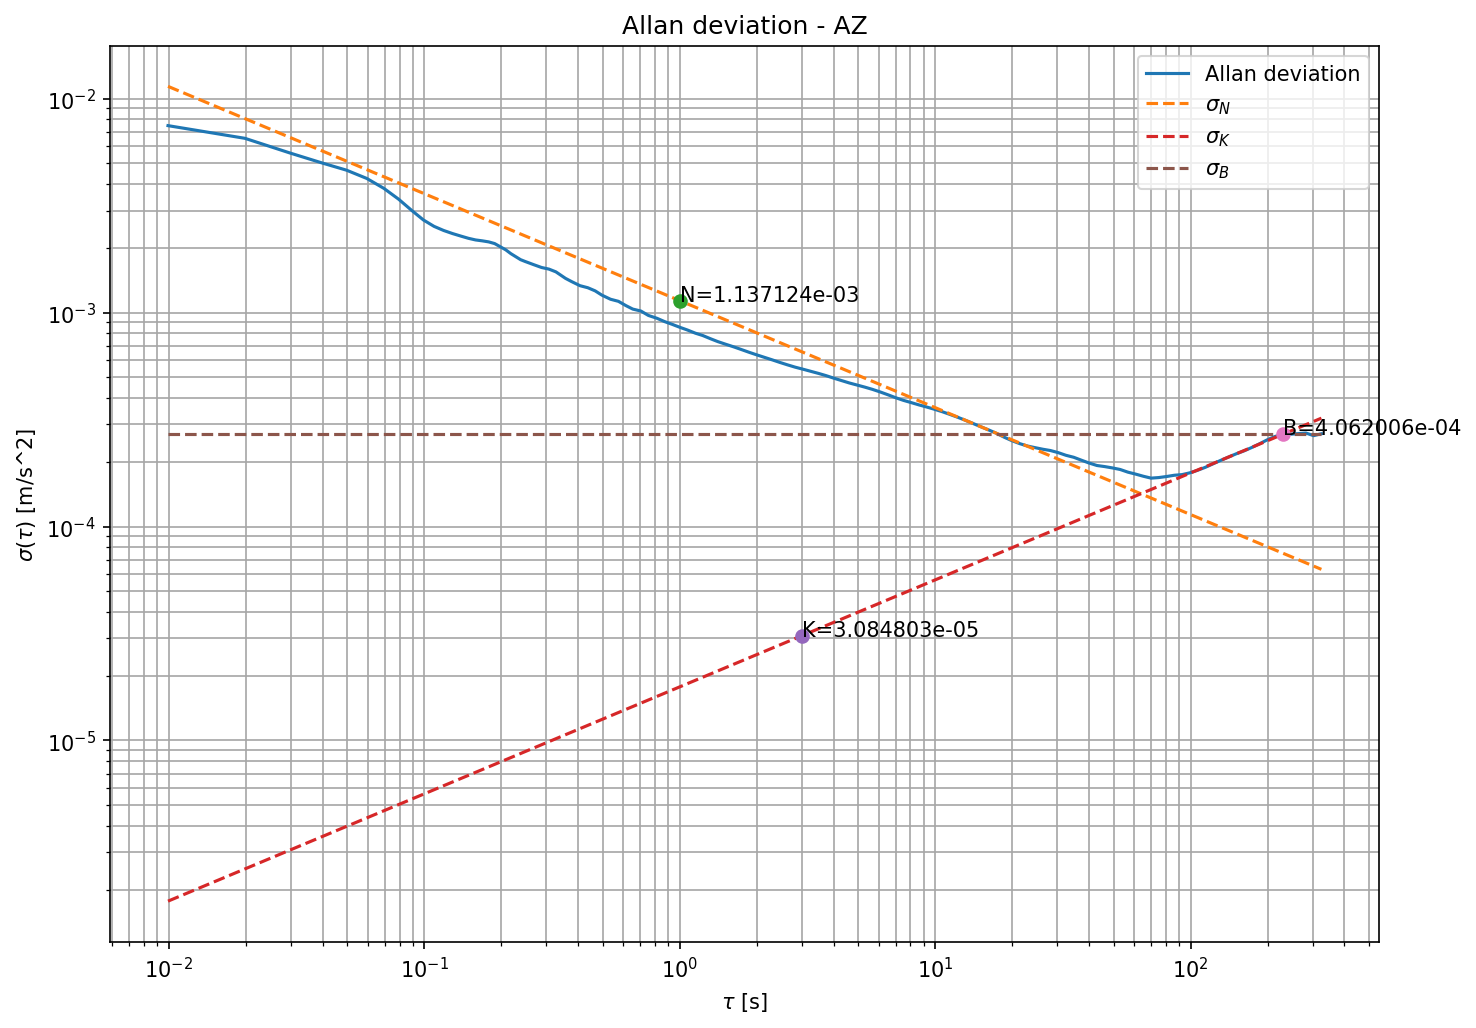
\includegraphics[width=0.88\textwidth]{images/az_allan.png}
    \caption{Curva de desviación de Allan correspondiente al eje \(z\) del acelerómetro durante el ensayo estático de una hora.}
    \label{fig:allan_az_anexo}
\end{figure}

\begin{figure}[p]
    \centering
    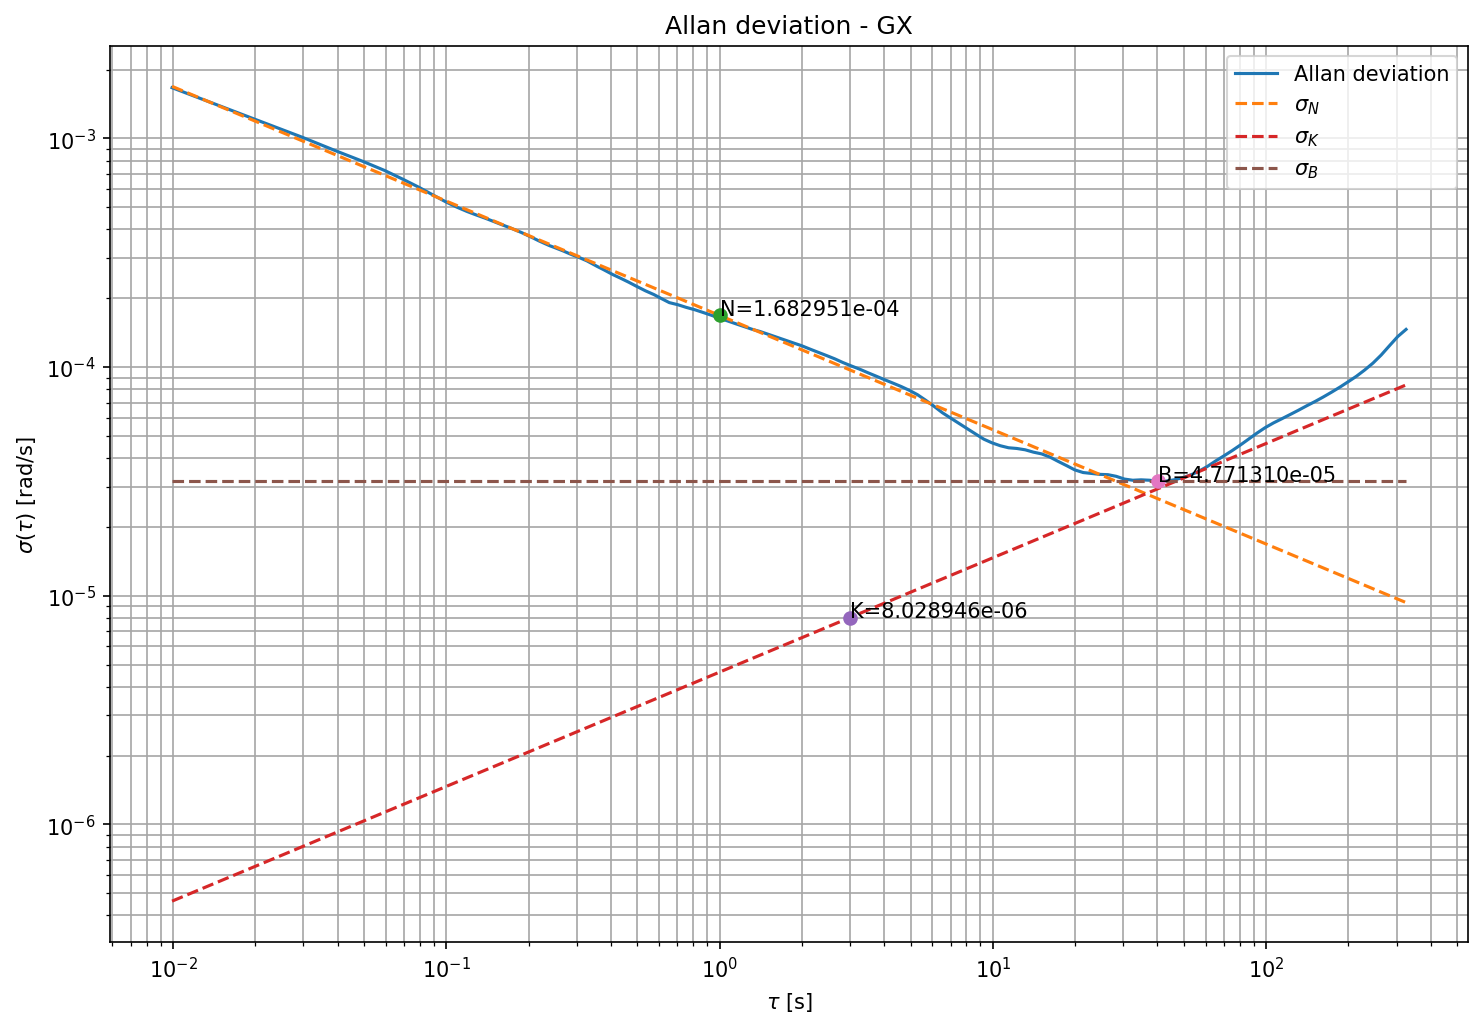
\includegraphics[width=0.88\textwidth]{images/gx_allan.png}
    \caption{Curva de desviación de Allan correspondiente al eje \(x\) del giróscopo durante el ensayo estático de una hora.}
    \label{fig:allan_gx_anexo}
\end{figure}

\begin{figure}[p]
    \centering
    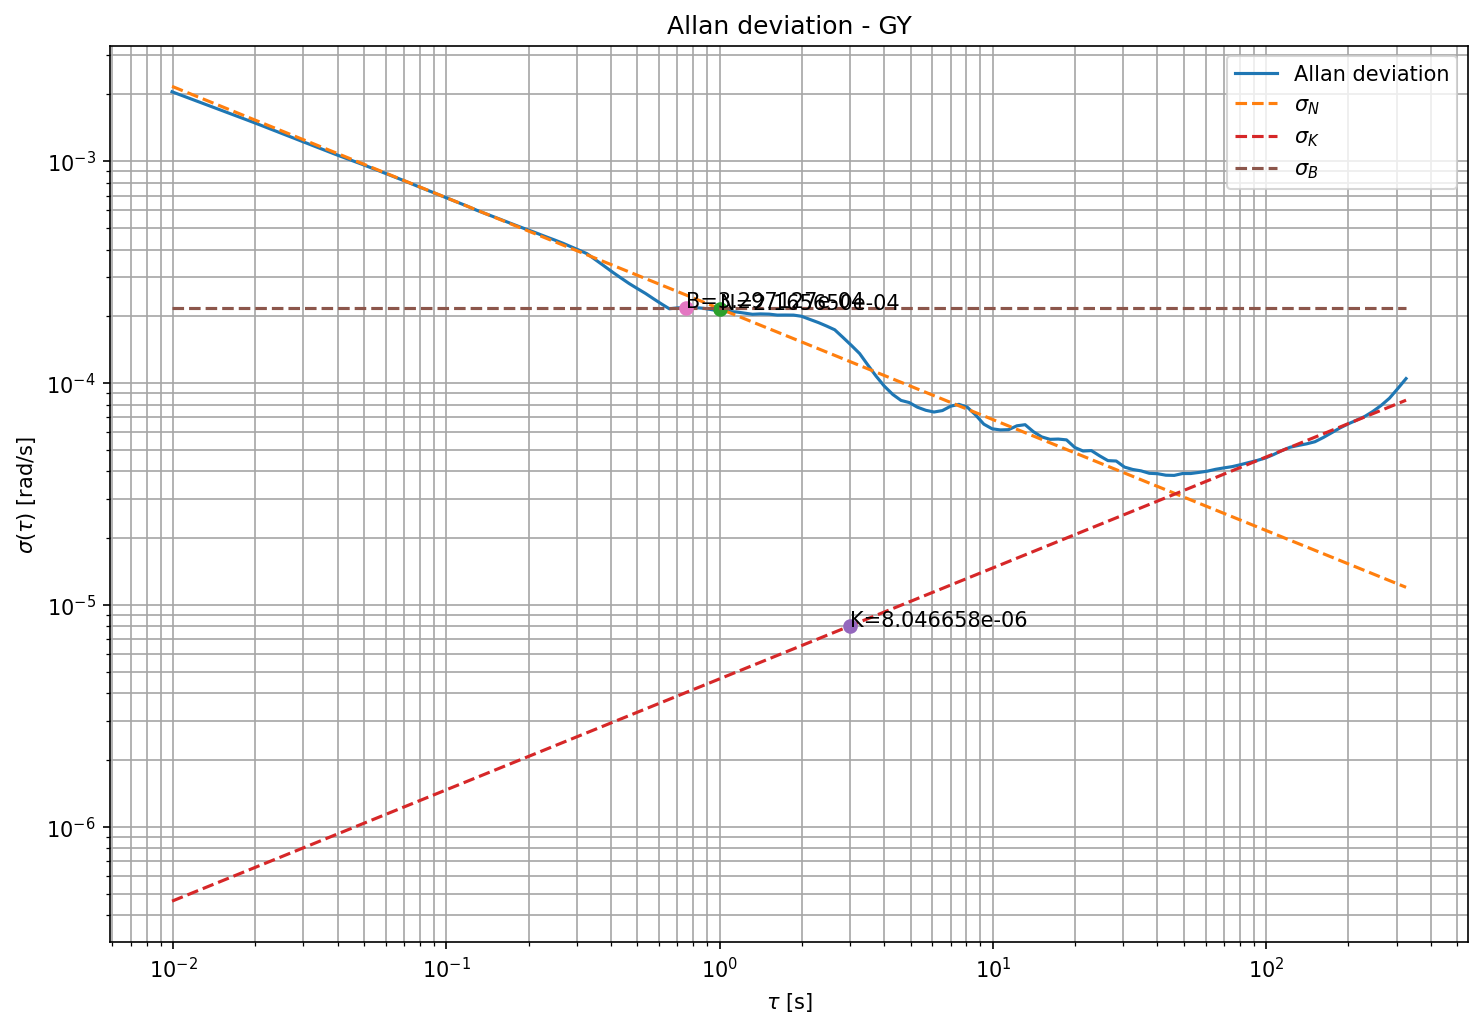
\includegraphics[width=0.88\textwidth]{images/gy_allan.png}
    \caption{Curva de desviación de Allan correspondiente al eje \(y\) del giróscopo durante el ensayo estático de una hora.}
    \label{fig:allan_gy_anexo}
\end{figure}

\begin{figure}[p]
    \centering
    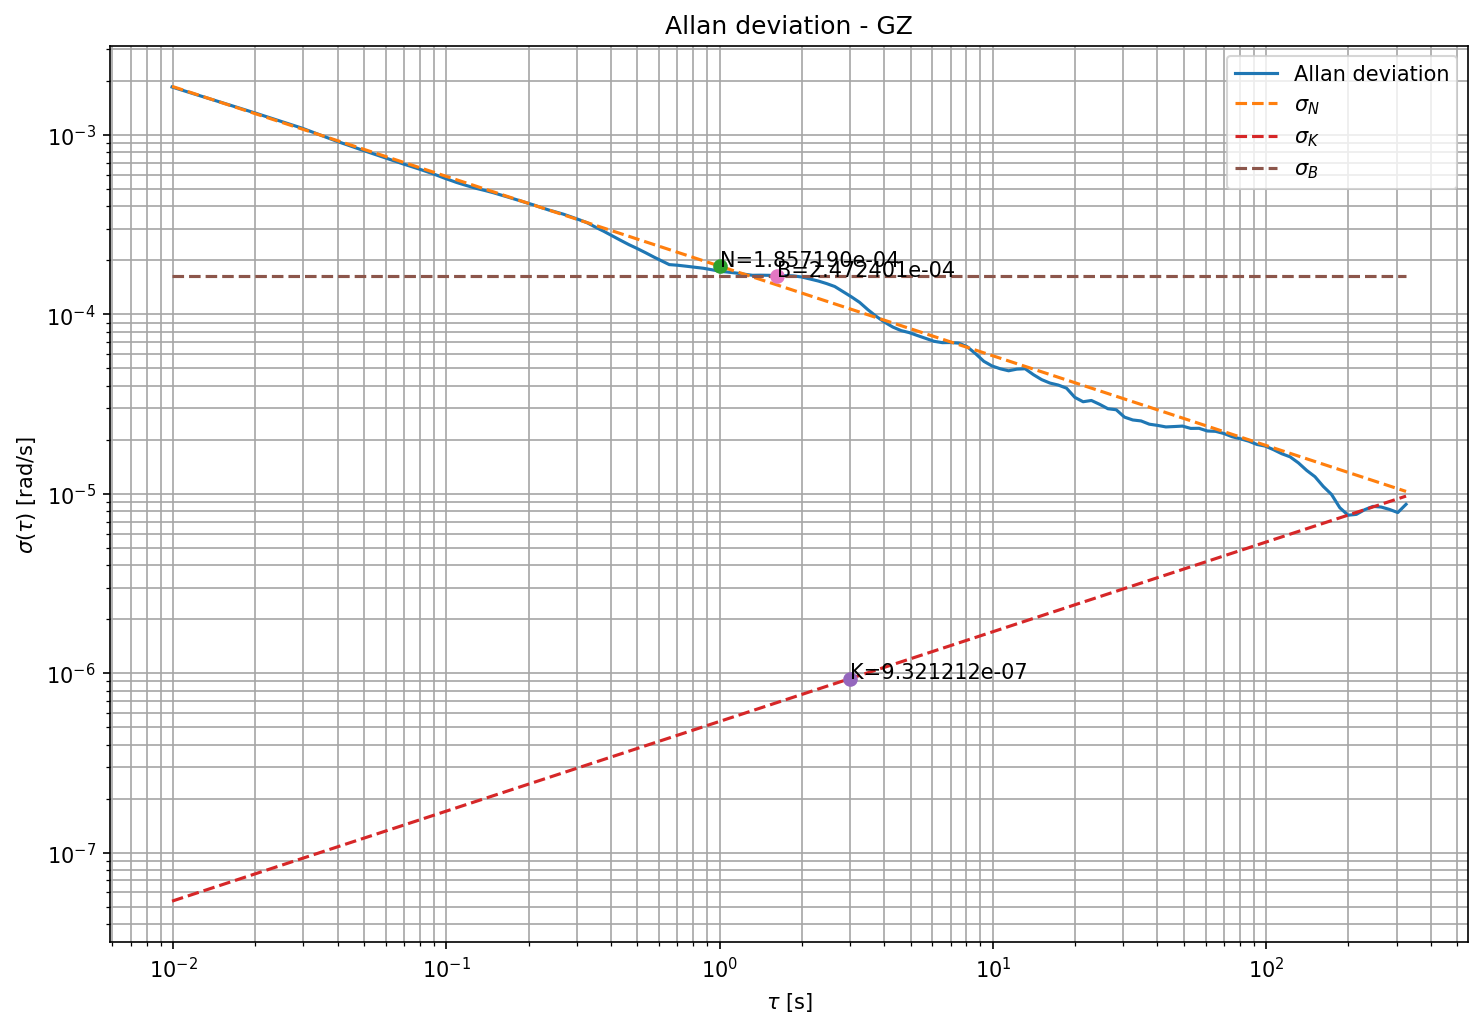
\includegraphics[width=0.88\textwidth]{images/gz_allan.png}
    \caption{Curva de desviación de Allan correspondiente al eje \(z\) del giróscopo durante el ensayo estático de una hora.}
    \label{fig:allan_gz_anexo}
\end{figure}